\section{NbAs}
\subsection*{Material ID: mp-dbf}
\textbf{Constante Dieléctrica ($\epsilon_{total}$):} 57262.63 \\[0.5em]
\begin{table}[h!]
\centering
\begin{tabular}{lcc}
\toprule
\textbf{Métrica} & \textbf{Lámina (Plate)} & \textbf{Cilindros (Rod)} \\
\midrule
Bandgaps ($a/\lambda$) & [0.700 - 0.720], [0.722 - 0.729], [0.731 - 0.751], [0.753 - 0.793], [0.795 - 0.822], [0.824 - 0.840] & [0.700 - 0.716], [0.718 - 0.748], [0.750 - 0.760], [0.762 - 0.768], [0.770 - 0.795], [0.797 - 0.812], [0.814 - 0.818], [0.820 - 0.835], [0.837 - 0.840] \\
Resonancias & 36 & 36 \\
\bottomrule
\end{tabular}
\end{table}
\begin{figure}[H]
\centering
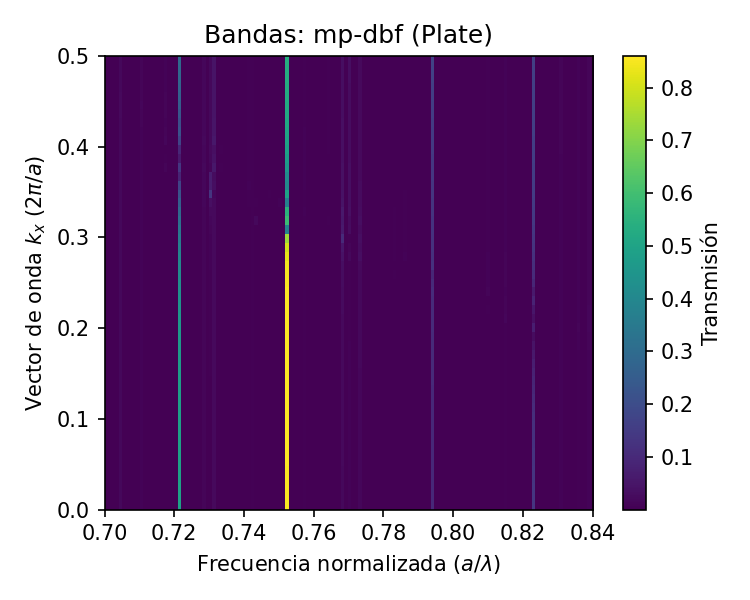
\includegraphics[width=0.48\textwidth]{figures/mp-dbf_plate.png}
\hfill
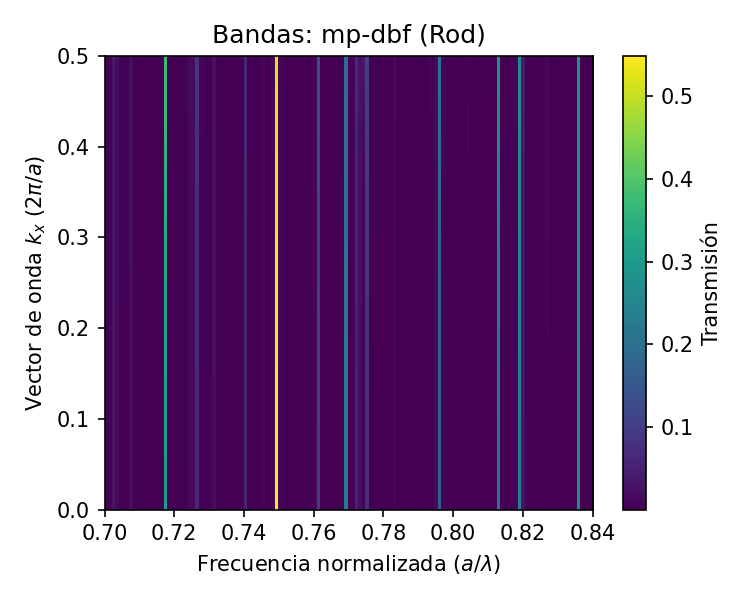
\includegraphics[width=0.48\textwidth]{figures/mp-dbf_rod.png}
\caption{Estructuras de bandas fotónicas para mp-dbf. Izquierda: Lámina. Derecha: Cilindros.}
\end{figure}
\vspace{1em}
\hrule
\vspace{1em}
\clearpage